% Created 2017-03-23 Thu 10:24
\documentclass[10pt,t,a4paper]{beamer}
\usepackage[utf8]{inputenc}
\usepackage[T1]{fontenc}
\usepackage{fixltx2e}
\usepackage{graphicx}
\usepackage{longtable}
\usepackage{float}
\usepackage{wrapfig}
\usepackage{rotating}
\usepackage[normalem]{ulem}
\usepackage{amsmath}
\usepackage{textcomp}
\usepackage{marvosym}
\usepackage{wasysym}
\usepackage{amssymb}
\usepackage{hyperref}
\tolerance=1000
\usetheme{BTH_msv}
\author{Mikael Svahnberg\thanks{Mikael.Svahnberg@bth.se}}
\date{2016-03-16}
\title{Requirements \\\\ Engineering}
\hypersetup{
  pdfkeywords={},
  pdfsubject={},
  pdfcreator={Emacs 25.1.1 (Org mode 8.2.10)}}
\begin{document}

\maketitle

\section{Classroom}
\label{sec-1}
\begin{frame}[fragile,label=sec-1-1]{Requirements Engineering \\ A Brief Overview}
 \begin{itemize}
\item Develop requirements through an iterative co-operative process of analysing the problem
\item Documenting the resulting observations in a variety of representation formats
\item checking the accuracy of the understanding gained
\end{itemize}

See the course \verb~PA1410 Requirements Engineering~
\end{frame}
\begin{frame}[label=sec-1-2]{Difficulties in Requirements Engineering}
\begin{itemize}
\item The customer may not be able to express what he or she wants so that you are able to understand it
\begin{itemize}
\item Tacit knowledge
\end{itemize}
\item Finding the right people to ask
\item Getting access to the right people
\item Handling large amounts of requirements
\item Specifying the requirements so that both you, the customer, your developers, and your testers can understand and use them
\end{itemize}
\end{frame}
\begin{frame}[label=sec-1-3]{Requirements Engineering Phases}
\begin{itemize}
\item Elicitation
\item Analysis \& Negotiation
\item Validation
\item Documentation
\item Management
\end{itemize}
\end{frame}
\begin{frame}[label=sec-1-4]{Discuss: RE Sources and Techniques}
\begin{itemize}
\item How do we find requirements?
\item Where do we find requirements?
\end{itemize}
\end{frame}
\begin{frame}[label=sec-1-5]{Requirements Elicitation Techniques}
\begin{itemize}
\item Interviews
\item Use-Case-based Discussions
\item Observations
\item Brainstorming
\item Questionnaires
\item Prototyping
\item Incremental Deliveries
\item Analysis of Written Documents
\end{itemize}
\end{frame}
\begin{frame}[label=sec-1-6]{Discuss: System Scope}
\begin{itemize}
\item What is the scope of the system?
\begin{itemize}
\item System boundaries
\end{itemize}
\item What should you do?
\item What should you not do?
\begin{itemize}
\item Balance: Requirements, Schedule and Budget
\end{itemize}
\item During Analysis / Design: Black Box vs White Box
\end{itemize}
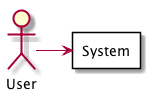
\includegraphics[height=3cm]{FScope.png}
\end{frame}

\begin{frame}[label=sec-1-7]{Requirements Specification}
\begin{itemize}
\item What the proposed system shall do
\begin{itemize}
\item At what quality level
\end{itemize}
\item A documented common view
\item An agreement between developers and customer
\begin{itemize}
\item Sign a contract based on the requirements specification
\end{itemize}
\item Involve client in process
\item Decrease Risk
\end{itemize}
\end{frame}
\begin{frame}[shrink=35,label=sec-1-8]{Quality Attributes}
\begin{columns}
\begin{column}{0.7\textwidth}
\begin{verse}
Accessibility, accountability, accuracy, adaptability, additivity, adjustability, affordability, agility, audiability, buffer, space performance, capability, capacity, clarity, code-space performance, cohesiveness, commonality, communication cost, communication time, compataibility, completeness, component integration time, component integration cost, composability, comprehensibility, conceptuality, conciseness, confidentiality, configurability, consistency, controllability, coordination cost, coordination time, correctness, cost, coupling, customer evaluation time, customer loyalty, customizability, data-space performance, decomposability, degradation of service, dependability, development cost, development time, deversity, distributivety, domain analysis cost, domain analysis time, efficiency, elasticity, enhanceability, evolvability, execution cost, extensibility, external cosistency, fault-tolerance, feasibility, flexibility, formality, generality, guidance, hardware cost, impact analyzability, independence, informativeness, inspection cost, inspection time, integrity, internal consistency, inter-operability, intuitiveness, learnability, main-memory performance, maintainability, maintenance cost, maintenance time, maturity, mean performance, measurability, mobility, modifiability, modularity, naturalness, nomadicity, obervability, off-peak-period performance, operability, operating cost, peak-period performance, performability, performance, planning cost, planning time, plasticity, portability, precision, predictability, process management time, productivity, project stability, project tracking cost, promptness, prototyping cost, prototyping time, reconfigurability, recoverability, recovery, reengineering cost, reliability, repeatability, replacability, replicability, response time, responsiveness, retirement cost, reusability, risk analysis cost, risk analysis time, robustness, safety, scalability, secondary-storage performance, sensitivity, security, similarity, simplicity, software cost, software production time, space boundness, space  performance, specificity, stability, standardizability, subjectivity, supportability, surety, survivability, susceptibility, sustainability, testability, testing time, throughput, time performance, timeliness, tolerance, tracebility, trainability, transerability, transparancy, understandability, uniform performance, uniformity, usability, user-friendliness, validity, variability, verifiability, versatility, visibility, wrappability \\
\end{verse}
\end{column}
\begin{column}{0.2\textwidth}
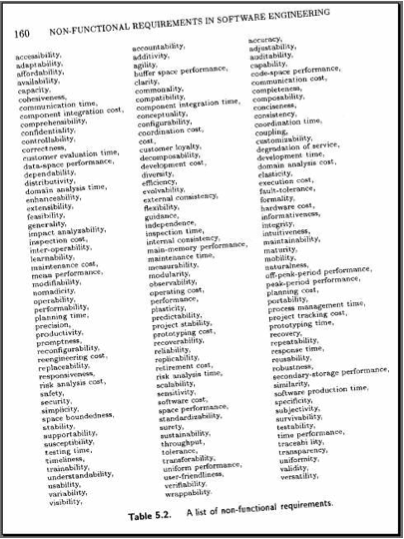
\includegraphics[width=9cm]{./IQualityAttributes.png}
\end{column}
\end{columns}
\end{frame}
\begin{frame}[label=sec-1-9]{More Structured Quality Attributes: \\ ISO9126}
\begin{itemize}
\item Functionality
\begin{itemize}
\item Suitability, Accuracy, Interoperability, Security, Functionality Compliance
\end{itemize}
\item Reliability
\begin{itemize}
\item Maturity, Fault Tolerance, Recoverability, Reliability Compliance
\end{itemize}
\item Usability
\begin{itemize}
\item Understandability, Learnability, Operability, Attractiveness, Usability Compliance
\end{itemize}
\item Efficiency
\begin{itemize}
\item Time Behaviour, Resource Utilisation, Efficiency Compliance
\end{itemize}
\item Maintainability
\begin{itemize}
\item Analysability, Changeability, Stability, Testability, Maintainability Compliance
\end{itemize}
\item Portability
\begin{itemize}
\item Adaptability, Installability, Co-Existence, Replaceability, Portability Compliance
\end{itemize}
\end{itemize}
\end{frame}
\begin{frame}[label=sec-1-10]{Discuss: Requirement Attributes}
\begin{itemize}
\item Requirements ID
\item Title
\item Description
\item Rationale
\item Restrictions \& Risks
\item Source
\item Fit Criterion / Test Case
\item Customer Priority
\item Dependencies
\end{itemize}
\begin{block}{Discuss}
What is the purpose of each of these attributes?
\end{block}
\end{frame}
\begin{frame}[label=sec-1-11]{Format of Requirements}
\begin{itemize}
\item What the system should do
\begin{itemize}
\item not how the system should do it
\end{itemize}
\item Testable - Measurable
\item Unambiguous
\item Only one requirement
\item Unique
\item Understood by all parties

\item Text, Figure, Diagram, Table?
\end{itemize}
\end{frame}
\begin{frame}[label=sec-1-12]{User Stories}
\begin{itemize}
\item Simpler template:
\begin{itemize}
\item As a \emph{type of user}, I want \emph{some goal} so that \emph{some reason}.
\end{itemize}
\item Written on index cards or post-it notes.
\item Often with \emph{acceptance tests} on the flip-side.
\end{itemize}
\end{frame}
\begin{frame}[label=sec-1-13]{Levels of Requirements}
T. Gorschek and C. Wohlin. Requirements abstraction model. \emph{Requirements Engineering}, 11:79–101, 2006:

\begin{itemize}
\item \alert{Goals} : Aligned with product Strategies
\item \alert{Features} : High-level descriptions of system functionalities
\item \alert{Functions} :  break-down of each feature
\item \alert{Components} : further breakdown
\end{itemize}

Do we see the system as a \emph{Black Box} or a \emph{White Box}?
\begin{description}
\item[{Black box}] What can we do towards the system, how does it respond?
\item[{White box}] What does the system do internally?
\end{description}
\end{frame}
\begin{frame}[label=sec-1-14]{Discuss: Good and Bad Examples}
\begin{itemize}
\item The system should be easy to use
\end{itemize}
\only<2>{
\begin{verse}
ID: Req.QA.Useability \\
Title: Useability for New Users \\
Description: The system shall be easy to learn for new users. \\
Rationale: The average user is not accustomed to using computers. \\
Source: Customer Meeting 2002-01-14, PG Gyllenhammar \\
Value Scale: Number of Hours it takes for a novice user to learn a new operation \\
Wanted value: 0,5 h / operation \\
Worst case value: 1,5 h / new operation \\
\end{verse}
}
\end{frame}
\begin{frame}[label=sec-1-15]{Discuss: Good and Bad Examples}
\begin{itemize}
\item The system should be stable
\item The user should be able to log in. If the user fails to log in after three attempts the user account should be locked.
\end{itemize}
\end{frame}
\begin{frame}[shrink=15,label=sec-1-16]{Customer Contacts}
\begin{itemize}
\item Respect
\item Responsibility
\item Commitment to the Customer
\item Credibility
\item Professional
\item Deliver at least what you have agreed upon
\begin{itemize}
\item Deliver at most?
\end{itemize}
\item Only one Customer? Only one Stakeholder?
\end{itemize}
\begin{block}{Customer Meetings}
\begin{itemize}
\item Be prepared
\item Have an Agenda
\item Document what is said
\item Reply quickly after a meeting with your perception of what was said
\begin{itemize}
\item e.g. in the form of a draft requirements specification
\end{itemize}
\item Act professional
\begin{itemize}
\item You are in control -- you should act like it
\end{itemize}
\end{itemize}
\end{block}
\end{frame}
\begin{frame}[label=sec-1-17]{Contracts}
\begin{itemize}
\item “A written judicial document defining the terms for business related agreements”
\begin{itemize}
\item Verbal agreements
\item Written agreements
\end{itemize}

\item Defines
\begin{itemize}
\item Deliverables
\item Payments
\end{itemize}

\item Written in sunshine, used in storm

\item Contract Types
\begin{itemize}
\item Fixed price
\item Running price
\item Cost-plus
\item Roof price
\item Combinations
\end{itemize}
\end{itemize}
\end{frame}
\begin{frame}[label=sec-1-18]{Contract Contents}
\begin{itemize}
\item Definition of Services
\item Time Period
\item Contact persons
\item Costs
\item Deliveries
\item General Conditions

\item Connected to:
\begin{itemize}
\item A Specific Version of the Requirements Specification
\item Project Plan?
\end{itemize}
\end{itemize}
\end{frame}
\begin{frame}[label=sec-1-19]{Contract: Important Points}
\begin{itemize}
\item The contract defines what you shall do.
\item The contract also defines what you can expect from the customer.
\item You sign the contract knowing that you can deliver what is specified, under the specified conditions.
\end{itemize}
\end{frame}
\begin{frame}[label=sec-1-20]{Back to RUP / Use Cases}
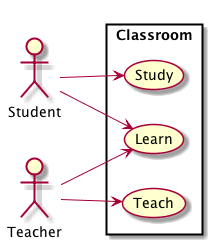
\includegraphics[height=6cm]{FUseCases.png}
\end{frame}

\begin{frame}[label=sec-1-21]{Discuss: Good and Bad Requirements II}
\emph{Users shall be able to view a personal calendar and recent notifications in the system.}

\begin{verse}
Use Case: View Calendar and Notifications \\
Actors: System Users \\
Description: \\
\hspace*{2em}A user requests to view their personal calendar. \\
\hspace*{4em}The system displays the users' personal calendar. \\
\hspace*{2em}A user requests to view their recent notifications. \\
\hspace*{4em}The system displays the users' recent notifications. \\
\end{verse}
\end{frame}
\begin{frame}[label=sec-1-22]{Discussion on Use Case Ranking}
\begin{block}{Increase ranking of a use case if it}
\begin{itemize}
\item has direct impact on architectural design
\begin{itemize}
\item example: adds classes to domain layer, require persistent services
\end{itemize}
\item includes risky, time-critical, complex functions
\item involves new research or technology
\item represents primary business processes
\item directly supports revenue or decreased costs
\end{itemize}
\end{block}
\begin{block}{Discuss}
For each of these cases, why does it increase the rank of a use case?
\end{block}
\end{frame}

\begin{frame}[label=sec-1-23]{Use Case Ranking Techniques}
\begin{itemize}
\item Scored (Numerical Weights)
\item Discrete (High, Medium, Low)
\item Simple Ordering (bubble sort?)
\item MoSCoW (Must have, Should have, Could have, Won't have)
\item Cumulative Voting
\end{itemize}
\end{frame}
% Emacs 25.1.1 (Org mode 8.2.10)
\end{document}